\documentclass{article}  
\usepackage{array}
% Include all project wide packages here.
\usepackage{fullpage}
\usepackage{polyglossia}
\setmainlanguage{english}
\usepackage{csquotes}
\usepackage{graphicx}
\usepackage{epstopdf}
\usepackage{pdfpages}
\usepackage{caption}
\usepackage[list=true]{subcaption}
\usepackage{float}
\usepackage{standalone}
\usepackage{import}
\usepackage{tocloft}
\usepackage{wrapfig}
\usepackage{authblk}
\usepackage{array}
\usepackage{booktabs}
\usepackage[toc,page,title,titletoc]{appendix}
\usepackage{xunicode}
\usepackage{fontspec}
\usepackage{pgfplots}
\usepackage{SIunits}
\pgfplotsset{compat=newest}
\pgfplotsset{plot coordinates/math parser=false}
\newlength\figureheight 
\newlength\figurewidth
\usepackage{unicode-math}
\usepackage[
    backend=bibtexu,
	texencoding=utf8,
bibencoding=utf8,
    style=ieee,
    sortlocale=nl_NL,
    language=auto
]{biblatex}
\usepackage{listings}
\newcommand{\includecode}[3][c]{\lstinputlisting[caption=#2, escapechar=, style=#1]{#3}}
\newcommand{\superscript}[1]{\ensuremath{^{\textrm{#1}}}}
\newcommand{\subscript}[1]{\ensuremath{_{\textrm{#1}}}}


\newcommand{\chapternumber}{\thechapter}
\renewcommand{\appendixname}{Bijlage}
\renewcommand{\appendixtocname}{Bijlagen}
\renewcommand{\appendixpagename}{Bijlagen}

\usepackage[hidelinks]{hyperref} %<--------ALTIJD ALS LAATSTE
  
\renewcommand{\familydefault}{\sfdefault}

\setmainfont[Ligatures=TeX]{Myriad Pro}
\setmathfont{Asana Math}
\setmonofont{Lucida Console}

\usepackage{titlesec, blindtext, color}
\definecolor{gray75}{gray}{0.75}
\newcommand{\hsp}{\hspace{20pt}}
\titleformat{\chapter}[hang]{\Huge\bfseries}{\chapternumber\hsp\textcolor{gray75}{|}\hsp}{0pt}{\Huge\bfseries}
\renewcommand{\familydefault}{\sfdefault}
\renewcommand{\arraystretch}{1.2}
\setlength\parindent{0pt}

%For code listings
\definecolor{black}{rgb}{0,0,0}
\definecolor{browntags}{rgb}{0.65,0.1,0.1}
\definecolor{bluestrings}{rgb}{0,0,1}
\definecolor{graycomments}{rgb}{0.4,0.4,0.4}
\definecolor{redkeywords}{rgb}{1,0,0}
\definecolor{bluekeywords}{rgb}{0.13,0.13,0.8}
\definecolor{greencomments}{rgb}{0,0.5,0}
\definecolor{redstrings}{rgb}{0.9,0,0}
\definecolor{purpleidentifiers}{rgb}{0.01,0,0.01}


\lstdefinestyle{csharp}{
language=[Sharp]C,
showspaces=false,
showtabs=false,
breaklines=true,
showstringspaces=false,
breakatwhitespace=true,
escapeinside={(*@}{@*)},
columns=fullflexible,
commentstyle=\color{greencomments},
keywordstyle=\color{bluekeywords}\bfseries,
stringstyle=\color{redstrings},
identifierstyle=\color{purpleidentifiers},
basicstyle=\ttfamily\small}

\lstdefinestyle{c}{
language=C,
showspaces=false,
showtabs=false,
breaklines=true,
showstringspaces=false,
breakatwhitespace=true,
escapeinside={(*@}{@*)},
columns=fullflexible,
commentstyle=\color{greencomments},
keywordstyle=\color{bluekeywords}\bfseries,
stringstyle=\color{redstrings},
identifierstyle=\color{purpleidentifiers},
}

\lstdefinestyle{matlab}{
language=Matlab,
showspaces=false,
showtabs=false,
breaklines=true,
showstringspaces=false,
breakatwhitespace=true,
escapeinside={(*@}{@*)},
columns=fullflexible,
commentstyle=\color{greencomments},
keywordstyle=\color{bluekeywords}\bfseries,
stringstyle=\color{redstrings},
identifierstyle=\color{purpleidentifiers}
}

\lstdefinestyle{vhdl}{
language=VHDL,
showspaces=false,
showtabs=false,
breaklines=true,
showstringspaces=false,
breakatwhitespace=true,
escapeinside={(*@}{@*)},
columns=fullflexible,
commentstyle=\color{greencomments},
keywordstyle=\color{bluekeywords}\bfseries,
stringstyle=\color{redstrings},
identifierstyle=\color{purpleidentifiers}
}

\lstdefinestyle{xaml}{
language=XML,
showspaces=false,
showtabs=false,
breaklines=true,
showstringspaces=false,
breakatwhitespace=true,
escapeinside={(*@}{@*)},
columns=fullflexible,
commentstyle=\color{greencomments},
keywordstyle=\color{redkeywords},
stringstyle=\color{bluestrings},
tagstyle=\color{browntags},
morestring=[b]",
  morecomment=[s]{<?}{?>},
  morekeywords={xmlns,version,typex:AsyncRecords,x:Arguments,x:Boolean,x:Byte,x:Char,x:Class,x:ClassAttributes,x:ClassModifier,x:Code,x:ConnectionId,x:Decimal,x:Double,x:FactoryMethod,x:FieldModifier,x:Int16,x:Int32,x:Int64,x:Key,x:Members,x:Name,x:Object,x:Property,x:Shared,x:Single,x:String,x:Subclass,x:SynchronousMode,x:TimeSpan,x:TypeArguments,x:Uid,x:Uri,x:XData,Grid.Column,Grid.ColumnSpan,Click,ClipToBounds,Content,DropDownOpened,FontSize,Foreground,Header,Height,HorizontalAlignment,HorizontalContentAlignment,IsCancel,IsDefault,IsEnabled,IsSelected,Margin,MinHeight,MinWidth,Padding,SnapsToDevicePixels,Target,TextWrapping,Title,VerticalAlignment,VerticalContentAlignment,Width,WindowStartupLocation,Binding,Mode,OneWay,xmlns:x}
}

%defaults
\lstset{
basicstyle=\ttfamily\small,
extendedchars=false,
numbers=left,
numberstyle=\ttfamily\tiny,
stepnumber=1,
tabsize=4,
numbersep=5pt
}  
\begin{document}

For the robot to get from one point to another manually, cameras are needed to see the surroundings and navigate through them. Furthermore, when the the robot needs to use its arm for a task it is convenient if there is a camera in the arm as well. This is because the point of view makes it easier to grab objects or drill in the right spot. The two camera options the team has is a CMOS image sensor or a CCD.



\subsection{CCD}

When a CCD, short for charge-coupled device, is exposed to light the small photosites on the surface of the CCD capture the light and store it in the form of a charge, as seen in figure \ref{ccd1} .

\begin{figure}[H]
	\centering
	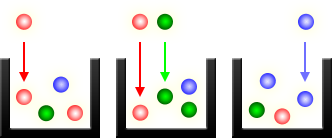
\includegraphics[scale=1]{figures/sensors_photosites-mono}
	\caption{Representation of photosites, charges are collected at the electrodes. }
	\label{ccd1}
\end{figure}


To read out the charge of each photosite a complete row is put into an amplifier one photosite at a time and after that the amplified signal is then passed on to an ADC, analog to digital converter. When the complete row has been read out the row above it moves one down, as do all the rows above, and then that row goes through the amplifier and ADC. This process is done until all rows are read and the image is now digital. This is also where the name comes from , charge-coupled device, because the rows of charges are coupled to the row above them. When one moves down all do. A visual representation is seen in figure \ref{ccd2}.

\begin{figure}[H]
	\centering
	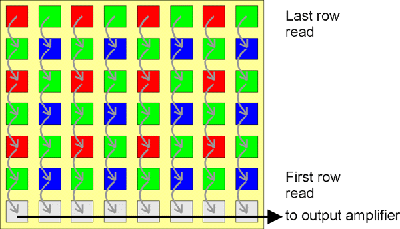
\includegraphics[scale=1]{figures/ccdreadout}
	\caption{Visual image of how the CCD reads out the array of photosites. This happens one row at a time.}
	\label{ccd2}
\end{figure}

The polysilicon electrodes on the surface of the chip are so small and close together that the charge is kept intact when physically moving from the place where the light was actually captured to the place where the signal is amplified. To achieve this a clock is needed to move all the charges at the same time, this needs to be done by an off-chip (or secondary chip). This is in order to not interfere with the closely packed polysilicon electrodes on the chip. 

Because the CCD needs extra circuitry which needs to be accurate, it can result in a very specified circuit with multiple power sources that need to operate at different, critical values which might not be regular. It is not rare for CCDs to have 5 or 6 of these power sources, this means that a lot of power is needed to operate the chip as intended.


\subsection{CMOS image sensor}

A newer technology is the CMOS image sensor, it can be easily incorporated with chips and other circuitry made on the same CMOS wafers. There are two basic types of CMOS image sensors, one being passive and the other active. The passive-pixel sensor works along the same principles as the CCD however now the circuitry is on the same chip as the sensors/photosites. This causes noise which can be seen on the image produced. The active-pixel sensors have extra circuitry at each pixel to cancel out the noise, this increases the quality of the image and makes it possible to go for higher resolutions. Here the performance can be equal to that of the CCDs. The negative side here is that this takes up extra space within the area of the photosites/pixels, see figure \ref{cmos1}. This results in the photosites not being as close to each other as they are at the CCDs for example (the fillfactor is lower compared to CCDs). Because there is less area capturing the light. This results in a lower charge thus a lower amplitude signal running through the ADC. For the image itself this results in a lower light intensity. This makes the image appear darker than it actually is and therefor makes the CMOS image sensor  less qualified to take images of dark environments.

\begin{figure}[H]
	\centering
	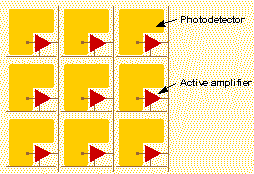
\includegraphics[scale=1]{figures/fillfactor}
	\caption{An abstraction of the circuitry around the photosites. }
	\label{cmos1}
\end{figure}



\subsection{Comparison}

CMOS imagers have a better intergration in circuits compared to the CCD cameras. Plus they use less power and are smaller. The negative here is that CMOS imagers have a lower image quality. Making them they less useful in high end image applications. Another negative for CMOS imagers compared to CCD cameras is that they are less flexible. This due to the circuitry already around the sensor, this is needed for it to work and cannot be changed while a CCD can be implemented in more systems. So the overall trend is that CMOS   imagers are used for lower end imaging applications and in mass production while their counterpart the CCD is more suitable for the high end imaging applications.



\end{document}